\documentclass[aspectratio=169,11pt]{beamer}

\usepackage[T1]{fontenc}
\usepackage[utf8]{inputenc}
\usepackage{lmodern}
\usepackage{booktabs}
\usepackage{array}
\usepackage{amsmath}
\usepackage{graphicx}
\usepackage{tikz}
\usetikzlibrary{arrows.meta,positioning}

\definecolor{navy}{HTML}{1F3864}
\definecolor{blu}{HTML}{2A78D6}
\definecolor{ora}{HTML}{EB6834}

\usetheme{default}
\setbeamertemplate{navigation symbols}{}
\setbeamercolor{structure}{fg=navy}
\setbeamercolor{normal text}{fg=black!90}
\setbeamerfont{frametitle}{series=\bfseries,size=\large}
\setbeamertemplate{frametitle}{%
  \vspace{5pt}\color{navy}\insertframetitle\par\vspace{-3pt}\color{navy}\rule{\linewidth}{0.6pt}}
\setbeamertemplate{footline}{%
  \hfill\color{black!50}\footnotesize ST-BMSE \textbullet{} Esther Muthui (223932) \hspace{1em} \insertframenumber\hspace{0.6cm}\vspace{5pt}}
\setbeamertemplate{itemize items}[circle]
\setbeamercolor{itemize item}{fg=navy}
\setbeamerfont{itemize/enumerate body}{size=\normalsize}
\setbeamerfont{itemize/enumerate subbody}{size=\small}
\setbeamersize{text margin left=0.9cm,text margin right=0.9cm}
\setbeamercolor{alerted text}{fg=ora!85!black}
\setbeamercolor{block title}{bg=navy,fg=white}
\setbeamercolor{block body}{bg=navy!7,fg=black}
\setbeamercolor{block title alerted}{bg=ora!85!black,fg=white}
\setbeamercolor{block body alerted}{bg=ora!10,fg=black}
\renewcommand{\arraystretch}{1.15}
\newcommand{\code}[1]{\texttt{#1}}
\newcommand{\hl}[1]{{\color{navy}\textbf{#1}}}

\begin{document}

% ---------------------------------------------------------------- 1 title
\begin{frame}[plain]
  \vfill
  {\color{navy}\fontsize{30}{34}\selectfont\bfseries ST-BMSE\par}
  \vspace{4pt}
  {\color{navy}\LARGE\bfseries Forecasting county-level conflict escalation in Kenya\par}
  \vspace{10pt}
  \rule{0.5\linewidth}{1pt}\par
  \vspace{8pt}
  {\large DSA 8401 Applied Machine Learning \textbullet{} Capstone presentation\par}
  \vspace{3pt}
  {\large Esther Muthui (223932) \textbullet{} Strathmore University \textbullet{} November 2026\par}
  \vfill
  {\footnotesize\color{black!60} A stacked ensemble with empirical-Bayes Markov features, evaluated on an untouched 2022--2024 test period.\par}
\end{frame}

% ---------------------------------------------------------------- 2 problem
\begin{frame}{Which Kenyan counties will escalate \emph{next} month?}
  \begin{itemize}\setlength{\itemsep}{7pt}
    \item \hl{Task:} for each of 47 counties, estimate $P(\text{escalation in month } t{+}1)$ using only what is known at month $t$.
    \item \hl{Output:} a calibrated probability and an alert flag, as \emph{decision support} for a human analyst, not an automated decision.
    \item \hl{Why:} early warning relies on slow, qualitative field reports that are hard to compare across counties.
    \item \hl{Unequal costs:} a missed escalation is worse than a false alarm, so the alert threshold minimises expected cost
  \end{itemize}
  \[
    \tau^\star=\arg\min_{\tau}\big[\,C_{FN}\,FN(\tau)+C_{FP}\,FP(\tau)\,\big],\qquad C_{FN}:C_{FP}=5:1 \;\;\text{(my assumption)}
  \]
\end{frame}

% ---------------------------------------------------------------- 3 data
\begin{frame}{The data are synthetic, built to the proposal's design}
  \begin{columns}[T]
    \column{0.47\textwidth}
    \textbf{What the file contains}
    \begin{itemize}\setlength{\itemsep}{3pt}
      \item 5{,}640 rows: 47 counties $\times$ 120 months (2015--2024)
      \item 13 columns, no missing values, no duplicate keys
      \item Label: \code{Conflict\_Escalation} (28\% overall)
      \item Indicators: social unrest, economic volatility, tension, response time, sentiment, conflict type
    \end{itemize}
    \column{0.50\textwidth}
    \begin{block}{What ``synthetic'' means here}
      \small
      \begin{itemize}\setlength{\itemsep}{2pt}
        \item Simulated county-month records, not observed ACLED or KNBS data
        \item Follows the proposal's design: 47 counties, monthly, 2022--2024 test period
        \item Results demonstrate the \emph{method}, not real conflict in Kenya
        \item Real ACLED and KNBS data: the planned next stage
      \end{itemize}
    \end{block}
  \end{columns}
\end{frame}

% ---------------------------------------------------------------- 4 evaluation
\begin{frame}{Evaluation runs forward in time, and the world shifts under it}
  \begin{columns}[T]
    \column{0.36\textwidth}
    \begin{itemize}\setlength{\itemsep}{5pt}
      \item \hl{Train} on targets up to 2019
      \item \hl{Validate} 2020--2021: meta-learner and threshold
      \item \hl{Test} 2022--2024, touched once
      \item No shuffling, no random $k$-fold
    \end{itemize}
    \vspace{6pt}
    \begin{alertblock}{Prior shift}
      \small Escalation rate: 20\% $\to$ 24\% $\to$ \textbf{43\%}
    \end{alertblock}
    \column{0.62\textwidth}
    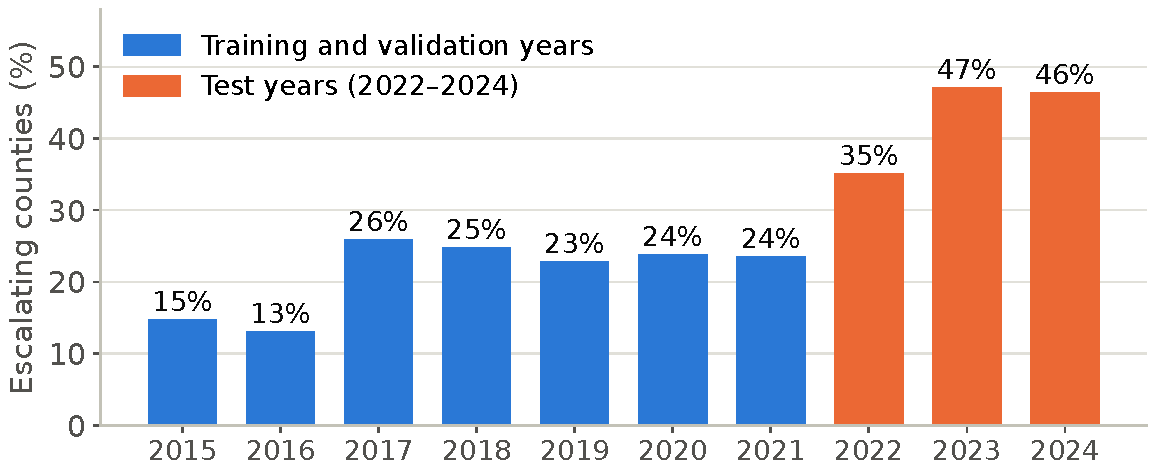
\includegraphics[width=\linewidth]{figures/fig_drift_s.pdf}
  \end{columns}
\end{frame}

% ---------------------------------------------------------------- 5 pipeline
\begin{frame}{A scripted, reproducible pipeline, served as an API}
  \centering
  \vspace{4pt}
  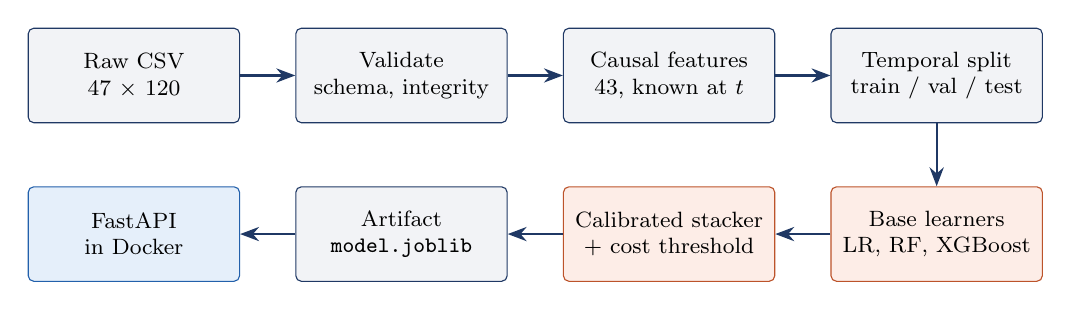
\begin{tikzpicture}[
    box/.style={draw=navy,fill=navy!6,rounded corners=2pt,minimum height=12mm,text width=2.45cm,align=center,font=\footnotesize},
    arr/.style={-{Stealth[length=2.4mm]},thick,navy},
    node distance=8mm and 7mm]
    \node[box] (a) {Raw CSV\\47 $\times$ 120};
    \node[box,right=of a] (b) {Validate\\schema, integrity};
    \node[box,right=of b] (c) {Causal features\\43, known at $t$};
    \node[box,right=of c] (d) {Temporal split\\train / val / test};
    \node[box,below=of d,fill=ora!12,draw=ora!80!black] (e) {Base learners\\LR, RF, XGBoost};
    \node[box,left=of e,fill=ora!12,draw=ora!80!black] (f) {Calibrated stacker\\+ cost threshold};
    \node[box,left=of f] (g) {Artifact\\\code{model.joblib}};
    \node[box,left=of g,fill=blu!12,draw=blu!80!black] (h) {FastAPI\\in Docker};
    \draw[arr] (a)--(b); \draw[arr] (b)--(c); \draw[arr] (c)--(d); \draw[arr] (d)--(e);
    \draw[arr] (e)--(f); \draw[arr] (f)--(g); \draw[arr] (g)--(h);
  \end{tikzpicture}
  \par\vspace{10pt}
  {\small One command reproduces everything: \code{python run\_pipeline.py}. Not notebook-based.\par}
\end{frame}

% ---------------------------------------------------------------- 6 features
\begin{frame}{Features use only what is known at month $t$}
  \begin{itemize}\setlength{\itemsep}{5pt}
    \item \hl{43 features:} escalation lags and 3/6/12-month shares, rolling indicators, calendar, one-hot categories
    \item \hl{Spill-over proxy:} escalation share of other counties in the same region (no adjacency data)
    \item \hl{Bayesian-Markov:} chance of escalating next month given the current state, shrunk toward the pooled rate
  \end{itemize}
  \[
    \hat p_{c,s,t}=\frac{n^{\to 1}_{c,s,t}+k\,\bar p_{s,t}}{n_{c,s,t}+k},\qquad k=10,\;\; \text{counts use transitions seen up to } t
  \]
  \begin{block}{Leakage guard (unit test)}
    \small Corrupt every observation after a cut-off month: no feature at or before it may change. The test caught two planted leaky features and left the real ones alone.
  \end{block}
\end{frame}

% ---------------------------------------------------------------- 7 models
\begin{frame}{Three learners, one calibrated blend, one cost-based threshold}
  \small
  \begin{tabular}{@{}>{\raggedright\arraybackslash}p{3.6cm}>{\raggedright\arraybackslash}p{9.6cm}@{}}
    \toprule \textbf{Technique} & \textbf{Why it fits} \\ \midrule
    Logistic regression & Interpretable baseline the proposal asks for; largest blend weight (0.48) \\
    Random forest & Non-linear interactions and region effects, little tuning \\
    XGBoost & Strong on structured tabular data \\
    Logistic stacker & Blends the three on the validation period and doubles as probability calibrator \\
    Cost-sensitive threshold & Encodes that a missed escalation costs more than a false alarm \\
    County-block bootstrap & Rows within a county are autocorrelated, so resample whole counties \\
    \bottomrule
  \end{tabular}
\end{frame}

% ---------------------------------------------------------------- 8 exclusions
\begin{frame}{What I deliberately left out, and one thing I simply did not do}
  \footnotesize
  \begin{tabular}{@{}>{\raggedright\arraybackslash}p{3.7cm}>{\raggedright\arraybackslash}p{9.5cm}@{}}
    \toprule \textbf{Not used} & \textbf{Reason} \\ \midrule
    LSTM / GRU / Transformer & 47 series of 120 points is too little data; interpretability suffers (argued, not tested) \\
    SVM, LightGBM & No expected gain over the learners already used \\
    K-Means, PCA, t-SNE & Task is supervised; clustering would not improve a one-month forecast \\
    LLM, RAG, agents & No text in the data \\
    SHAP & Not installed; permutation importance used instead (SHAP is the natural next step) \\
    \midrule
    \textbf{Hyperparameter search} & \textbf{Not done. Hyperparameters were fixed, not tuned. This is a limitation.} \\
    \bottomrule
  \end{tabular}
\end{frame}

% ---------------------------------------------------------------- 9 results
\begin{frame}{The ensemble beats the persistence baseline}
  \centering
  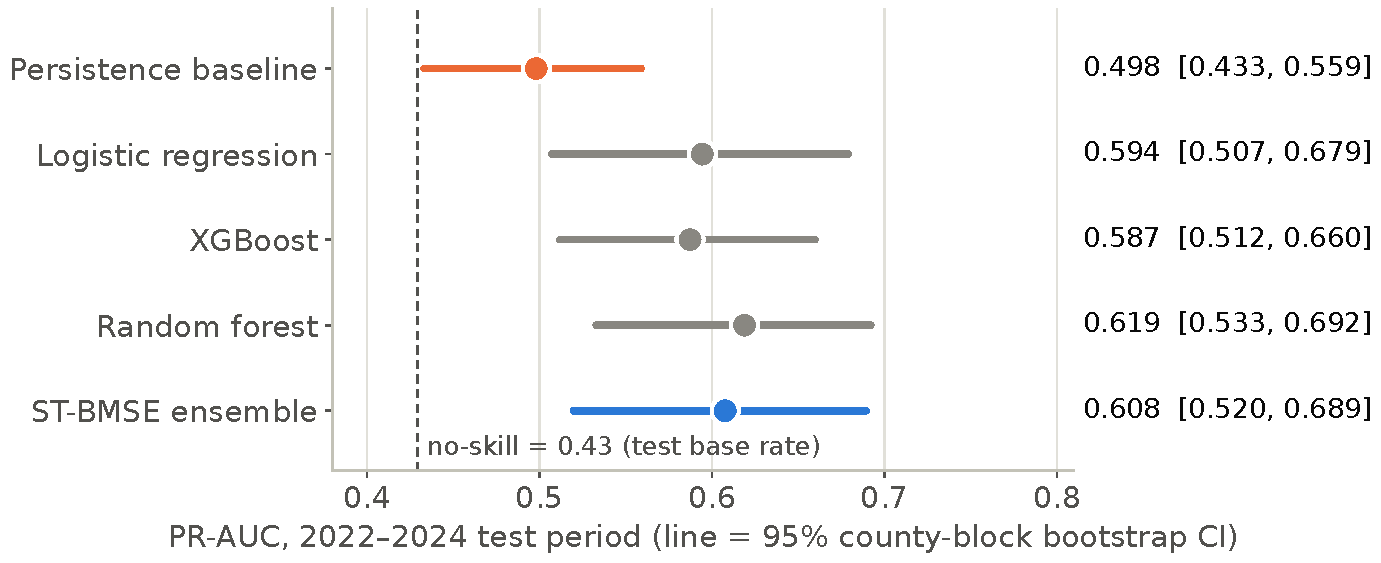
\includegraphics[width=0.92\linewidth]{figures/fig_results_s.pdf}
  \par\vspace{2pt}
  {\small Paired gain over persistence: \hl{+0.109 PR-AUC} (95\% CI 0.062 to 0.161), so it is outside noise.\par}
\end{frame}

% ---------------------------------------------------------------- 10 honest comparison
\begin{frame}{\ldots but it does not beat a single random forest}
  \small
  \begin{tabular}{@{}lccl@{}}
    \toprule \textbf{PR-AUC difference} & \textbf{Estimate} & \textbf{95\% CI} & \textbf{Reading} \\ \midrule
    Ensemble $-$ persistence & $+0.109$ & $0.062$ to $0.161$ & Real improvement \\
    Ensemble $-$ random forest & $-0.011$ & $-0.031$ to $+0.016$ & No evidence of a gain \\
    Ensemble $-$ logistic regression & $+0.013$ & $0.002$ to $0.026$ & Small, borderline \\
    \bottomrule
  \end{tabular}
  \normalsize
  \begin{itemize}\setlength{\itemsep}{6pt}
    \item The proposal's claim that stacking helps is \alert{not supported} on this data.
    \item ROC-AUC is about 0.69: moderate discrimination, not strong.
    \item Calibration is acceptable (ECE 0.049); Brier 0.221 against 0.383 for persistence.
  \end{itemize}
\end{frame}

% ---------------------------------------------------------------- 11 leakage
\begin{frame}{Same-month features nearly give the answer: a leakage audit}
  \centering
  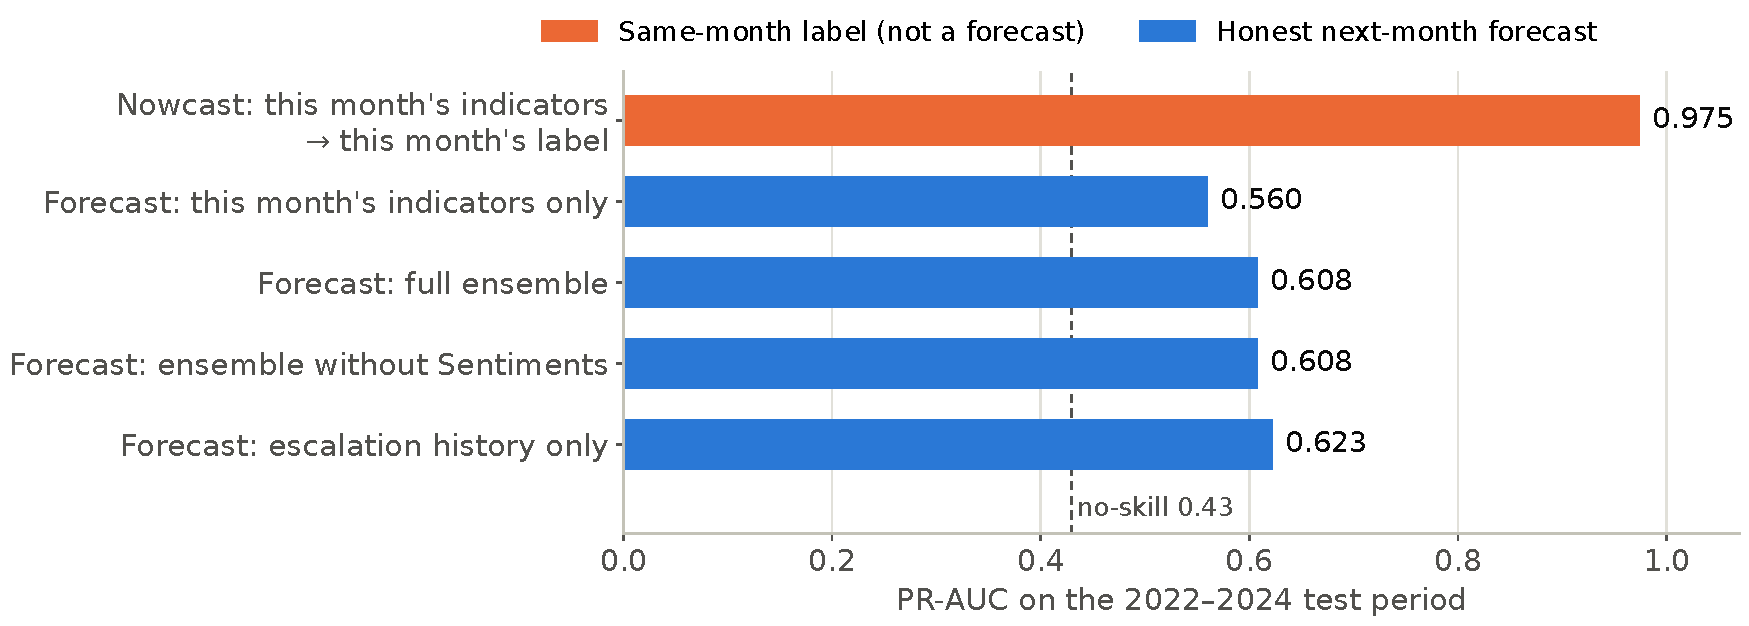
\includegraphics[width=0.9\linewidth]{figures/fig_leakage_s.pdf}
  \par\vspace{2pt}
  {\small \code{Sentiments}: 0\% escalation when Positive or Neutral, 83\% when Negative, \emph{in the same month}. A random split would look near-perfect.\par}
\end{frame}

% ---------------------------------------------------------------- 12 alert
\begin{frame}{The tuned alert flags almost every county}
  \begin{columns}[T]
    \column{0.55\textwidth}
    \begin{itemize}\setlength{\itemsep}{6pt}
      \item Threshold 0.18 was tuned on 2020--2021, when 24\% of months escalated.
      \item In the 43\% test regime: recall 0.94, \alert{false-alarm rate 0.81}.
      \item Latest month (Dec 2024): \alert{46 of 47 counties alert} at 0.18, 8 of 47 at 0.50.
      \item The API exposes a \code{threshold} override; the right value must be set with practitioners.
    \end{itemize}
    \column{0.42\textwidth}
    \begin{alertblock}{Takeaway}
      \small An alert that fires for everyone is noise. Thresholds tuned in one regime do not transfer to another.
    \end{alertblock}
  \end{columns}
\end{frame}

% ---------------------------------------------------------------- 13 fairness
\begin{frame}{False alarms fall unevenly across regions}
  \centering
  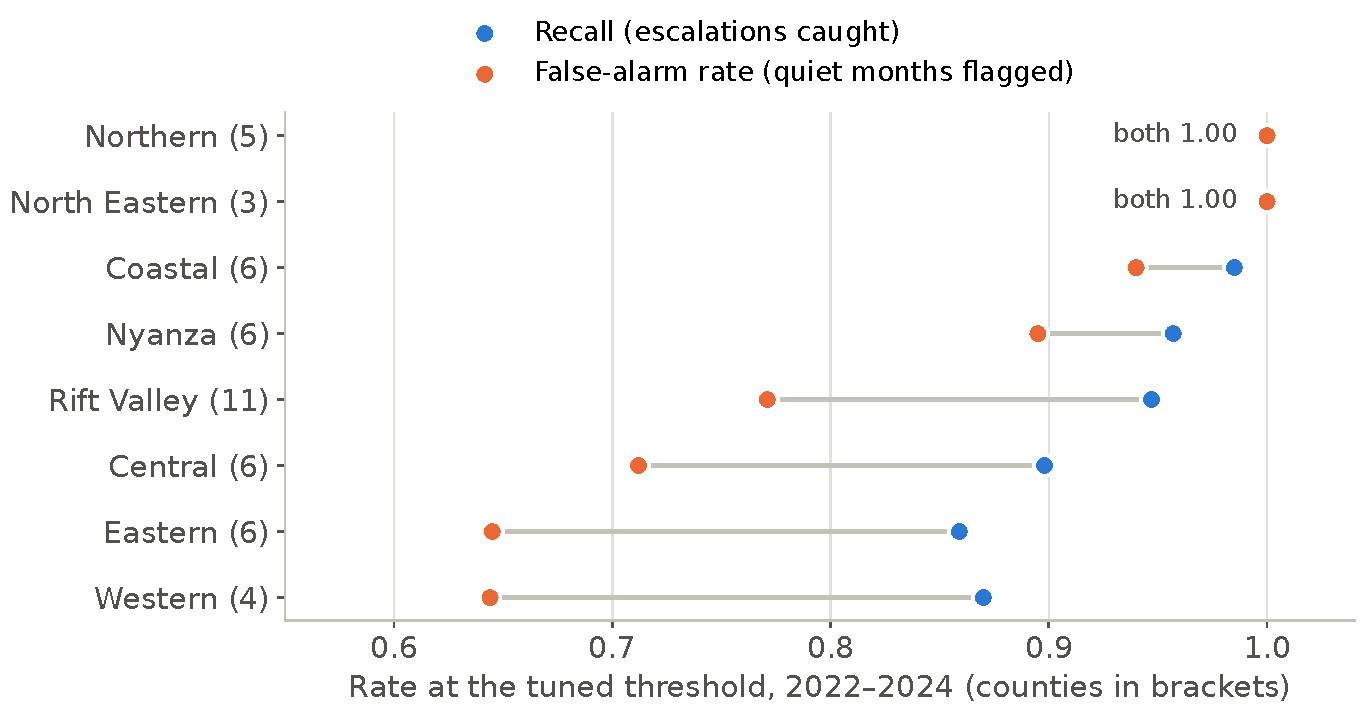
\includegraphics[width=0.84\linewidth]{figures/fig_region_s.pdf}
  \par\vspace{2pt}
  {\small Regions hold only 3 to 11 counties, so the differences are indicative, not conclusive.\par}
\end{frame}

% ---------------------------------------------------------------- 14 calibration
\begin{frame}{Probabilities are usable, but the base rate is drifting}
  \begin{columns}[c]
    \column{0.40\textwidth}
    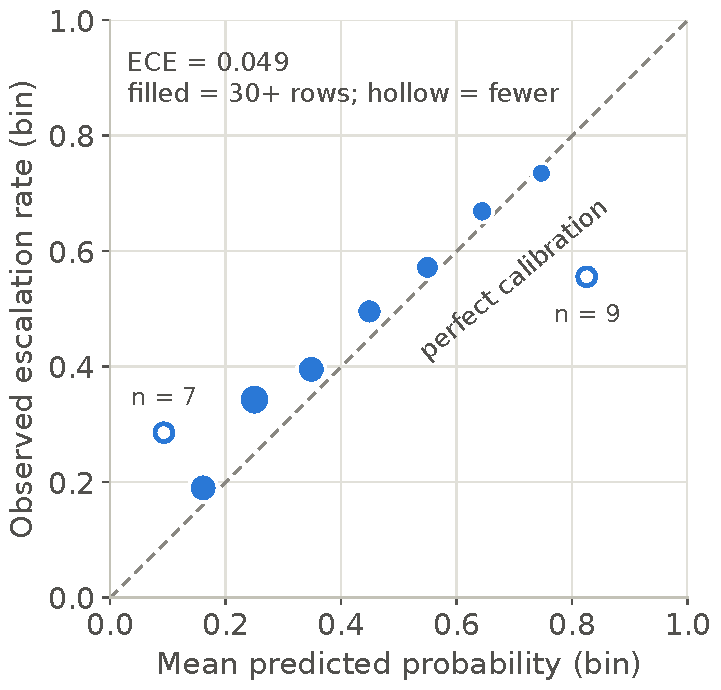
\includegraphics[width=\linewidth]{figures/fig_calibration_s.pdf}
    \column{0.56\textwidth}
    \begin{itemize}\setlength{\itemsep}{6pt}
      \item Expected calibration error \hl{0.049}.
      \item Slightly too low in low bins: the test base rate exceeds the training one.
      \item 18 continuous features have PSI above 0.25 between training and test.
      \item \hl{Implication:} retrain and re-tune the threshold on recent data.
    \end{itemize}
  \end{columns}
\end{frame}

% ---------------------------------------------------------------- 14b evidently
\begin{frame}{Evidently confirms it: 27 of 32 columns drifted, including the predictions}
  \begin{columns}[T]
    \column{0.55\textwidth}
    \textbf{Training period vs test period}
    \begin{itemize}\setlength{\itemsep}{4pt}
      \item \hl{27 of 32 columns (84\%)} drifted; dataset drift detected
      \item \alert{Prediction drift}: score 1.31 against a 0.1 threshold
      \item Target drift flagged (0.17): the base rate moved
      \item Biggest input shifts: spill-over shares, social-unrest score
    \end{itemize}
    \column{0.42\textwidth}
    \begin{block}{Sanity check passed}
      \small Month-of-year, region and response time did \emph{not} drift, as they should not.
    \end{block}
    \begin{block}{What it does not say}
      \small Inputs moved; accuracy is measured separately on labelled test data.
    \end{block}
  \end{columns}
  \vspace{4pt}
  {\footnotesize Agrees with the hand-built PSI check (18 features above 0.25). Full report: \code{reports/evidently\_drift\_report.html}.\par}
\end{frame}

% ---------------------------------------------------------------- 14c mlops
\begin{frame}{Every run is tracked and gated, and CI/CD ships only what passes}
  \small
  \begin{tabular}{@{}>{\raggedright\arraybackslash}p{2.7cm}>{\raggedright\arraybackslash}p{10.5cm}@{}}
    \toprule
    \textbf{MLflow} & Parameters, metrics, tables and model per run; the three learners as nested runs; passing model registered as \code{production} \\
    \textbf{Quality gate} & Validation only: best learner must beat persistence by $\ge 0.05$ PR-AUC. Fail $\to$ exit 1, no model saved, nothing registered \\
    \textbf{Proof} & Real data passes ($+0.179$). Demanding $+0.90$ stopped the pipeline with exit code 1 and left the registry untouched \\
    \textbf{CI} & Each push: train + gate, audits, Evidently, 32 tests, Docker build, run the container and call it \\
    \textbf{CD} & Push to the container registry only from the default branch, and only if CI passed \\
    \bottomrule
  \end{tabular}
  \vspace{6pt}
  \begin{alertblock}{Honest status}
    \small \textbf{Ran green on GitHub on its first push}, both jobs. Not verified: the published image was not listed independently, the file was not linted, and the gate's blocking was proven locally.
  \end{alertblock}
\end{frame}

% ---------------------------------------------------------------- 15 deployment
\begin{frame}{Served as an API in Docker, verified end to end}
  \begin{columns}[T]
    \column{0.47\textwidth}
    \textbf{FastAPI endpoints}
    \begin{itemize}\setlength{\itemsep}{2pt}\small
      \item \code{POST /predict}: one county
      \item \code{POST /predict/batch}: ranked list
      \item \code{GET /health}, \code{/model-info}
      \item Bad input $\to$ HTTP 422; unknown county $\to$ 404
    \end{itemize}
    \column{0.50\textwidth}
    \textbf{What I verified}
    \begin{itemize}\setlength{\itemsep}{2pt}\small
      \item 32 pytest tests pass
      \item Slim image builds (gate runs inside the build)
      \item Container \emph{healthy}, non-root; 200 and 422 over HTTP
    \end{itemize}
  \end{columns}
  \vspace{6pt}
  \begin{alertblock}{Reproducibility caveat}
    \small XGBoost is not bit-identical across Windows and Linux: ensemble PR-AUC 0.609 vs 0.608, but tuned threshold 0.16 vs 0.18.
  \end{alertblock}
\end{frame}

% ---------------------------------------------------------------- 15b frontend
\begin{frame}{An analyst view, served by the same API}
  \centering
  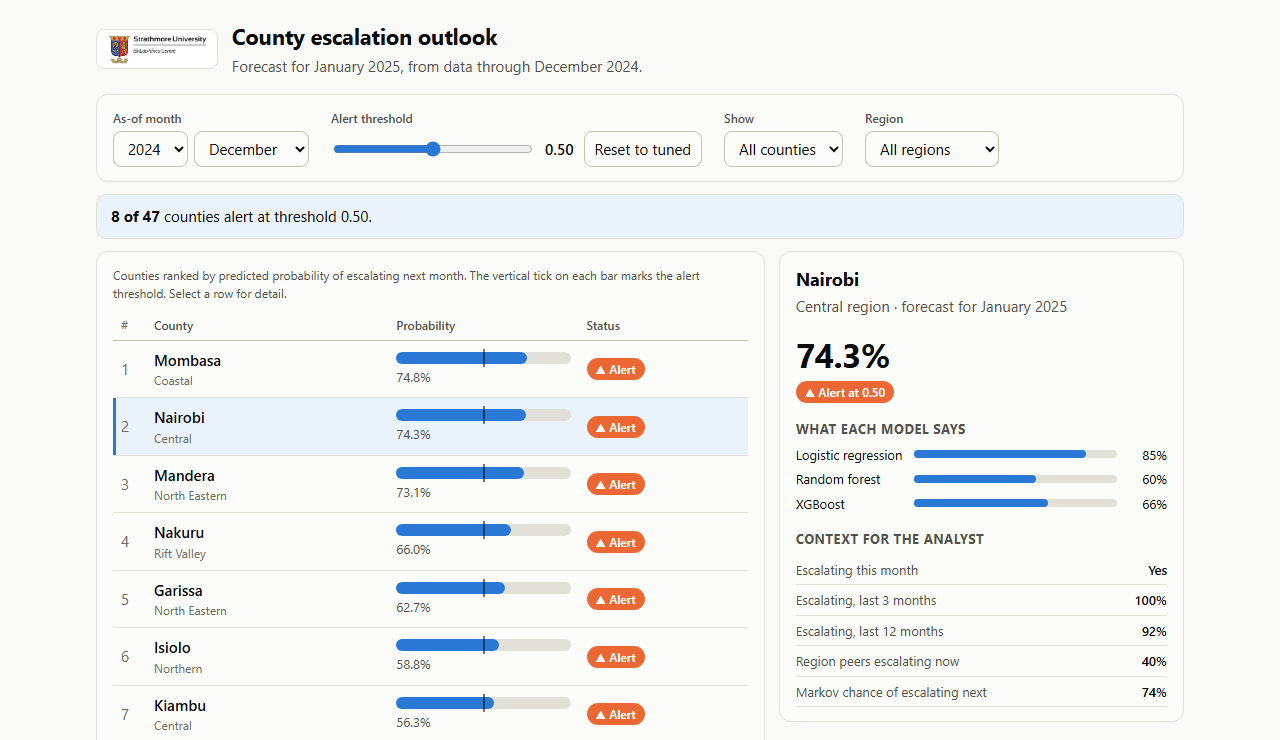
\includegraphics[width=0.70\linewidth]{figures/ui_screenshot.png}
  \par\vspace{2pt}
  {\small Threshold raised to 0.50 here: 8 of 47 counties alert. At the tuned 0.18 nearly every county alerts, and the page warns the analyst.\par}
\end{frame}

% ---------------------------------------------------------------- 16 gap
\begin{frame}{Where the delivery departs from the proposal}
  \footnotesize
  \begin{tabular}{@{}>{\raggedright\arraybackslash}p{5.3cm}>{\raggedright\arraybackslash}p{7.9cm}@{}}
    \toprule \textbf{Proposal} & \textbf{Delivered} \\ \midrule
    ACLED events and KNBS indicators & Synthetic county-month data; real data is the next stage \\
    Spatial spill-over from neighbours & Same-region share as a proxy \\
    Data-quality problems to be handled & Not present: synthetic data are complete \\
    Escalation is rare (class imbalance) & Common: 28\% overall, 43\% in test \\
    Stacking expected to outperform & Not shown; ties a random forest \\
    Dashboard integration & API with analyst context; no dashboard \\
    \bottomrule
  \end{tabular}
\end{frame}

% ---------------------------------------------------------------- 17 limits / next
\begin{frame}{Limitations, and what comes next}
  \begin{columns}[T]
    \column{0.48\textwidth}
    \textbf{Limitations}
    \begin{itemize}\setlength{\itemsep}{3pt}\small
      \item Synthetic data: no real-world claims
      \item One split; no rolling-origin evaluation
      \item Hyperparameters not tuned
      \item CI/CD ran once; workflow not linted
      \item 5:1 cost ratio and 0.05 gate margin assumed
      \item No causal claim
    \end{itemize}
    \column{0.48\textwidth}
    \textbf{Next}
    \begin{itemize}\setlength{\itemsep}{3pt}\small
      \item Real ACLED and KNBS data, with an explicit escalation definition
      \item Rolling-origin validation and tuning
      \item SHAP explanations; lint the workflow
      \item Threshold set with practitioners
    \end{itemize}
  \end{columns}
\end{frame}

% ---------------------------------------------------------------- 18 end
\begin{frame}[plain]
  \vfill
  \centering
  {\color{navy}\fontsize{30}{34}\selectfont\bfseries Questions\par}
  \vspace{12pt}
  {\large Code, tests, Docker files and report are in the project repository.\par}
  \vspace{4pt}
  {\small\color{black!60} \code{python run\_pipeline.py} \textbullet{} \code{docker compose up --build}\par}
  \vfill
\end{frame}

\end{document}
